\subsection{Дифракционная решетка}
\begin{minipage}{0.45\textwidth}
    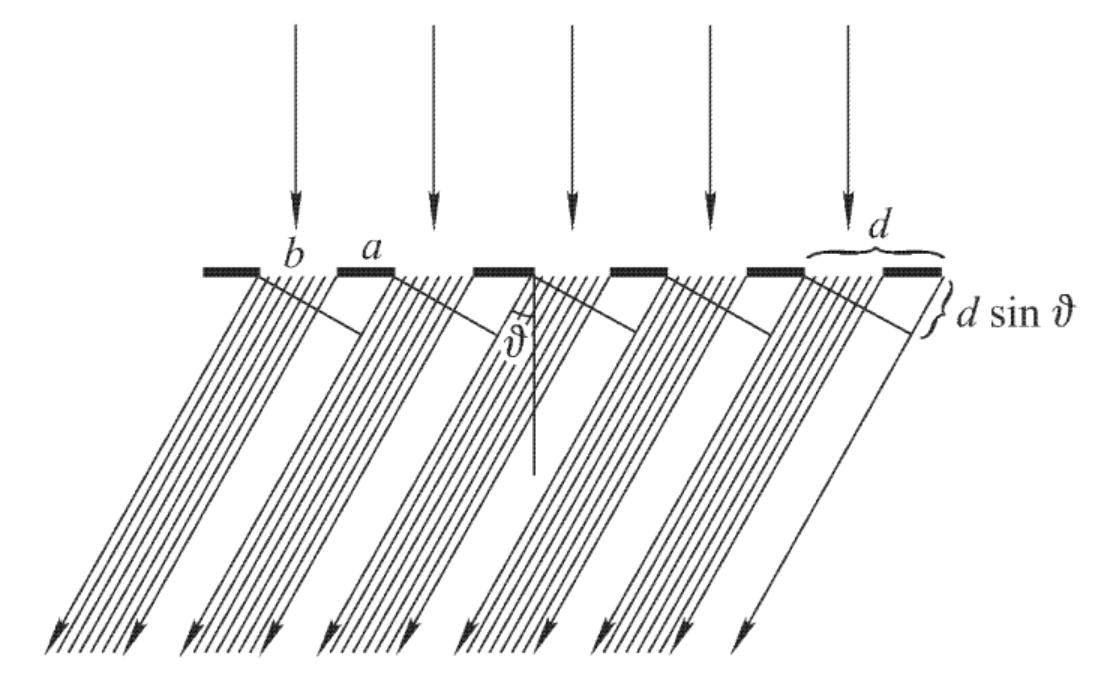
\includegraphics[width=1\textwidth]{figures/s36_1.png}
\end{minipage}
\hfill
\begin{minipage}{0.45\textwidth}
	Имеем простейший случай: лучи падают перпендикулярно, $d$ -- \textit{период решетки}, $\vartheta$ -- угол дифракции.
	Разность хода между волнами, исходящими из соседних щелей 
	\begin{equation*}
		\Delta = d \sin \vartheta, 	
	\end{equation*}
	а разность фаз 
	\begin{equation*}
		\delta = k d \sin \vartheta = 2 \pi d \sin \vartheta / \lambda.
	\end{equation*}  
	Поле, наблюдаемое от первой щели определяется формулой
	\begin{equation*}
		E_1 = \frac{b \sin\alpha}{\alpha}.
	\end{equation*}
\end{minipage}

Поля же излучаемые остальными щелями:
\begin{equation*}
	E_2 = E_1 e^{-i \delta}, 
	\hspace{0.5 cm}
	E_3 = E_1 e^{-2i \delta},
	\hspace{0.5 cm}
	\ldots
	\hspace{0.5 cm}
	E_N = E_1 e^{- i (N-1)\delta}.
\end{equation*}
Полное поле представится как сумма всех:
\begin{equation*}
	E = E_1 \frac{1- e^{- i N \delta}}{1 - e^{-i\delta}} = E_1 \frac{\sin \left(\frac{N \delta}{2}\right)}{\sin \left(\frac{\delta}{2}\right)}e^{- i (N-1)\delta/2}
	\hspace{1 cm}
	\Rightarrow
	\hspace{1 cm}
	I = I_1 \left[\frac{\sin \left(\frac{N \delta}{2}\right)}{\sin \left(\frac{\delta}{2}\right)}\right]^2.
\end{equation*}
Заметим, что при  
\begin{equation*}
	\delta/2 = m \pi
	\hspace{1 cm}
	\Leftrightarrow
	\hspace{1 cm}
	d \sin \vartheta = m \lambda.
\end{equation*}
получаем $I = N^2 I_1$ -- \textit{главные максимумы}, где $m$ -- целое число, \textit{порядок главного максимума}. Это соотношение так же определяет направление $\vartheta$ на главные максимумы.

Если у решетки $a = b$, то все главные максимумы четных порядков вообще не появятся, то есть из условия решетки получим условие для минимума на одной щели для $I_1=0$:
\begin{equation*}
	d \sin \vartheta = 2 n \lambda
	\hspace{1 cm}
	\Rightarrow
	\hspace{1 cm}
	b \sin \vartheta = n \lambda.
\end{equation*}
Таким образом в рассматриваемом направлении ни одна щель, а потому и решетка в целом не излучают.